\chapter{Input and output}

A number of years ago, Jeannette Wing published a terrific editorial with the title {\it Computational Thinking}, or in her own words, ``Ways to Think Like a Computer Scientist'' (see Communications of the ACM, March 2006).
This 3-page article summarizes many of the problem-solving techniques you will discover while learning to program.
Everyone interested in learning computer science beyond programming should read it.
She defines the field this way:

\index{computer science}

\begin{quote}
{\bf ``Computer science is the study of computation---what can be computed and how to compute it.''}
\end{quote}

So far the only programs we've looked at simply display messages, which doesn't involve a lot of real computation.
But that will change quickly as we begin to work with more types of data.
This chapter will show you how to read input from the keyboard, use that input to calculate a result, and then format that result for output.
We will also look at some technical details about how operating systems work.


\section{The Java class library}

\index{library}

Like most programming languages, Java has an extensive {\bf library} of class and method definitions that you can use in your programs.
You can browse this library on Oracle's website:
\url{http://docs.oracle.com/javase/7/docs/api/}

\index{package}

The standard edition of Java comes with {\em several thousand} classes, which can be both exciting and intimidating.
To help keep things organized, classes are grouped into {\bf packages}.
Just as each \java{class} is a separate file, each \java{package} is a separate folder.
We have now seen all major organizational units of Java code.
As a review from the previous two chapters:

\begin{figure}[!h]
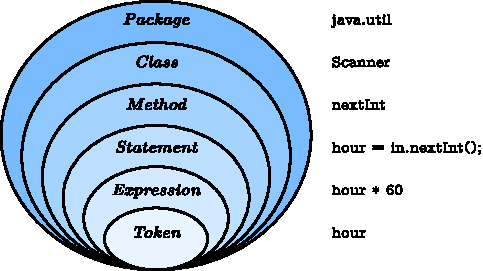
\includegraphics[width=4in]{package.pdf}
\caption{Elements of the Java language, from largest to smallest.}
\end{figure}

Two library classes we have used thus far, \java{System} and \java{String}, belong to the \java{java.lang} package.
According to the documentation, \java{java.lang} ``provides classes that are fundamental to the design of the Java programming language.''
Note there is a major difference between the Java {\em language}, which deals with syntax and grammar, and the Java {\em library}, which provides the built-in classes.
In fact, most of the Java library itself is written in Java!

\index{import}
\index{statement!import}

In order to use a class defined in another package (and in another folder), you have to {\bf import} it first.

\begin{code}
import java.io.File;
import java.io.PrintStream;
import java.util.Date;
import java.util.Scanner;
\end{code}

All \java{import} statements appear at the top of the source file, above the class definition.
It's not uncommon for Java programs to have many import statements.
Because they are so fundamental, all classes in \java{java.lang} are imported automatically.
That is why we haven't needed the \java{import} statement until now.

\subsection{The System class}
\label{sec:system}

\index{System class}
\index{class!System}
\index{object}

When you call \java{System.out.println}, you are referring to the \java{out} variable declared in the \java{System} class.
The \java{out} variable's type is \java{PrintStream}, which provides methods for ``printing'' data.
Both \java{System} and \java{PrintStream} are written in Java, and later in the book we'll examine their source code.
For now, you should understand that \java{System.out} is a \java{PrintStream} {\bf object}.
Because Java is an {\em object-oriented} language, much of the library is organized around objects that perform specific actions.

\begin{figure}[!h]
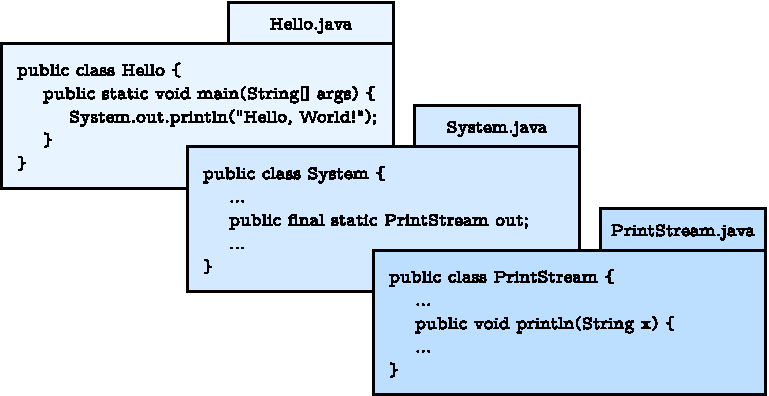
\includegraphics{system.pdf}
\caption{\java{System.out.println} references the \java{out} variable of the \java{System} class,
\\ which has the type \java{PrintStream}, which has a method called \java{println}.}
\end{figure}

\index{operating system}

As with most software, Java programs run on top of an {\bf operating system} that manages the keyboard, the display, main memory, disk drives, printers, the network, and other hardware resources.
Common examples of operating systems include Android, iOS, Linux, Mac OS~X, and Windows.
When starting Java programs, the operating system directs \java{System.out} to the screen.

\java{System.out} can display the value of any type of variable.
Indeed, you can even use \java{System.out} to print the value of \java{System.out}:

\begin{code}
System.out.println(System.out);
\end{code}

The result is:

\begin{stdout}
java.io.PrintStream@685d72cd
\end{stdout}

\index{address}

When Java prints an object, it prints the type of the object (\java{PrintStream}), the package where the type is defined (\java{java.io}), and the {\bf address} or location of the object in memory (after the \java{@} sign).
In this example the address is \java{685d72cd}, but if you run the same code you will likely get something different.
You can think of the address as a unique identifier for the object.

\index{abstraction}

Note the exact type of display doesn't matter, whether it's a 5-inch touch screen or 30-inch monitor.
From the programmer's point of view, \java{System.out} simply provides the means for printing messages.
Computer scientists often use {\bf abstraction} to deal with the complexity of software.
The \java{System} class is a platform-independent abstraction of the operating system.
The operating system itself is a layer of abstraction on top of computer hardware.

There is also an object named \java{System.in} that makes it possible to get input from the keyboard.
As with \java{System.out}, the exact type of keyboard (or even touch screen) does not matter to the programmer.
Unfortunately, Java does not make it easy to use \java{System.in} directly.
Instead, it provides other classes that make use of \java{System.in} for you.

\subsection{The Scanner class}

\index{Scanner class}
\index{class!Scanner}
\index{byte}

From the operating system's point of view, data from the keyboard arrives in a series of hardware control signals.
The operating system translates these signals into a stream of {\bf bytes} (small integers), which in turn need to be translated into characters.
\java{System.in} provides the means for reading one byte of input at a time, which is hardly useful for programs that would rather read in an entire word or line of input.

\index{class!utility}
\index{utility class}

That's where \java{java.util.Scanner} comes in handy.
\java{Scanner} is a {\bf utility class} that parses an input stream into words, lines, numbers, and other types of data.
Because \java{Scanner} belongs to the \java{java.util} package, you need to import it at the top of your program.
Otherwise you will get a compiler error like ``cannot find symbol'' (i.e., the compiler doesn't know what you mean by \java{Scanner}).

\begin{code}
import java.util.Scanner;
\end{code}

In most programs, you will need only one \java{Scanner}, since there is only one source of input.
The following code declares a \java{Scanner} variable and then creates a \java{Scanner} object that will parse \java{System.in}.

\begin{code}
    Scanner in;
    in = new Scanner(System.in);
\end{code}

\index{initialize}

As we saw previously with constants, it is also legal to declare a variable and initialize it at the same time:

\begin{code}
    Scanner in = new Scanner(System.in);
\end{code}

This latter syntax is more convenient, since it's a one-time setup for many programs.
Just make sure you understand that it's two statements in one.

At this point, you can use the variable \java{in} instead of \java{System.in}.
The following example reads two lines of input from the keyboard and repeats them back again to the user.

\begin{code}
import java.util.Scanner;

public class Echo {

    public static void main(String[] args) {
        String line;
        Scanner in = new Scanner(System.in);

        System.out.print("Type something:");
        line = in.nextLine();
        System.out.println("You said: " + line);

        System.out.print("Type something else:");
        line = in.nextLine();
        System.out.println("You also said: " + line);
    }

}
\end{code}


\section{Reading documentation}
\label{sec:apidocs}

\index{documentation}

Now would be a good time to take a look at the documentation for \java{Scanner}.
You can find it in the Java library (see the link earlier in this chapter) or simply do a web search for ``java scanner.''
The latter method is more useful in the long run, especially as Oracle releases new versions of Java.
Either way, you should get something like this:

\begin{figure}[!h]
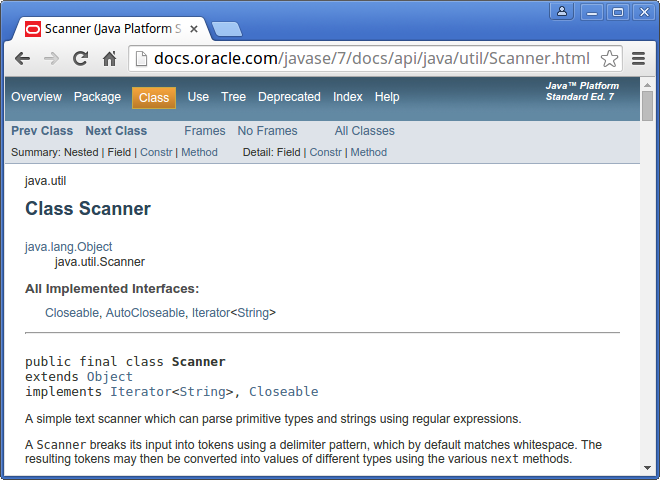
\includegraphics[width=\textwidth]{scanner.png}
\caption{Screenshot of the documentation for \java{Scanner} on Oracle's website.}
\end{figure}

Scroll down to the ``Method Summary'' section.
As you can see, the \java{Scanner} class provides quite a few methods.
In this chapter we'll focus on the ``next'' methods.
For example, click on the link for \java{nextInt}.

\begin{stdout}
public int nextInt()

Scans the next token of the input as an int.
\end{stdout}

\index{prototype}

The first line is the method's {\bf prototype}, which specifies the name of the method and its return type.
In this example, \java{nextInt} returns an \java{int}.
The next line describes what the method does.
The subsequent lines (not shown) explain the parameters and return values.
Explanations are often redundant, but the documentation is supposed to fit this standard format.
%The last line describes the exceptions this method might throw.

It might take some time to get comfortable reading this kind of information, but it's well worth the effort.
Knowing what methods a class provides helps you avoid reinventing the wheel.
Whenever you learn about a new class, you should take a quick look at its documentation.
On that note, take a few minutes to review the documentation for \java{System} and \java{String}.


\section{Writing documentation}

\index{Javadoc}

A nice feature of the Java language is the ability to write documentation at the same time you are writing the source code.
That way, the documentation stays in sync with the classes and methods themselves.
In fact, the HTML pages you browsed in the previous section were automatically generated using a tool called {\bf Javadoc}.
This tool is part of the standard JDK, and you can run it directly from DrJava by pressing the {\tt Javadoc} button on the toolbar.

\index{comments!documentation}
\index{documentation comments}

Javadoc parses your source files for {\bf documentation comments} and extracts other relevant information about your class and method definitions.
Given the prevalence of this tool, people sometimes refer to documentation as ``Javadoc comments.''
In contrast to inline comments that begin with {\tt //}, documentation comments begin with {\tt /**} (two stars) and end with {\tt */} (one star).
Anything in between these two tokens becomes part of the documentation.
As a rule of thumb, you should document every class and every method.

\begin{code}
/**
 * Example program that demonstrates print vs println.
 */
public class Goodbye {

    /**
     * Application entry point; simply prints a greeting.
     */
    public static void main(String[] args) {
        System.out.print("Goodbye, ");  // note the space
        System.out.println("cruel world");
    }

}
\end{code}

This example has perhaps too many comments, since all the program does is print a message.
But it illustrates the differences between inline and documentation comments:

\begin{itemize}
\item Inline comments tend to be short phrases that help explain complex parts of a method.
Documentation comments are typically complete sentences that begin with a capital letter and end with a period.

\item Documentation comments often span multiple lines.
By convention, each line begins with a {\tt *} that is aligned vertically with the start and end of the comment.

\item Some development environments (e.g., Eclipse and NetBeans) automatically display documentation comments when you hover your mouse over the name of a class or method.

\end{itemize}

Writing documentation and inline comments is essential for making source code readable.
As we discussed in the last chapter, people spend the majority of their development time understanding and modifying existing code.
You should not only write good comments for others, but for yourself as well.
When you haven't looked at your own code for a while, it takes a long time to remember how it works (or what you were trying to do) if there's no comments.


\section{Inches to centimeters}

An everyday problem that computers are great at solving is converting numbers from one unit into another.
Although most of the world has adopted the metric system for weights and measures, some countries are stuck with English units.
For example, when talking with friends in Europe about the weather, people in the United States may have to convert from Celsius to Fahrenheit and back.
And when making an international purchase online, you may have to convert your nation's currency into another based on the exchange rate.

%For the rest of the chapter, we will look at how to write programs that solve these types of problems.
%Specifically, each program will 1) prompt the user for input, 2) read input from the keyboard, 3) calculate a result, and 4) format the result for output.
%The focus will not only be on Java syntax and language features, but also on the {\em process} of solving the problem, documenting the code, and testing the solution.

Let's think about how to write this type of program.
This time, we'll even ask the user to input a specific value.
We'll need some variables and a scanner.

\begin{code}
    int inch;  // the input
    double cent;  // the output
    Scanner in = new Scanner(System.in);
\end{code}

The first step is to prompt the user for the input.
We'll use \java{print} instead of \java{println} so they can enter the input on the same line.

\begin{code}
    // prompt the user and get the value
    System.out.print("How many inches? ");
    inch = in.nextInt();
\end{code}

Next we multiply the number of inches by 2.54, since that's how many centimeters there are per inch.
Finally we display the results on one line, but use two print statements since it's easier to read.

\begin{code}
    // convert and output the result
    cent = inch * 2.54;
    System.out.print(inch + " in = ");
    System.out.println(cent + " cm");
\end{code}

\index{magic number}

This code works, but for readability we should get rid of the {\bf magic number}.
Let's put that 2.54 into a constant with a name that documents its purpose.

\begin{code}
    // convert and output the result
    final double centPerInch = 2.54;
    cent = inch * centPerInch;
    System.out.print(inch + " in = ");
    System.out.println(cent + " cm");
\end{code}

\subsection{Formatting output}

When printing floating-point numbers, Java automatically decides how many decimal places to display.

\begin{code}
    System.out.print(7.0 / 3.0);
    // prints 2.3333333333333335   note: 5 is a rounding error
\end{code}

\index{printf}

You can use \java{System.out.printf} to limit (or format) the number of decimal places.
Instead of just printing what is between the parentheses, \java{printf} allows for substitutions and formatting of output.
For example:

\begin{code}
    System.out.printf("%.3f", 7.0 / 3.0);
    // prints 2.333
\end{code}

The \java{printf} method takes two or more parameters, separated by commas.
The first parameter is a {\em format string}.
It contains a template for the text you want to output, as well as positions where it will substitute other values.

\begin{code}
    // what we had before
    System.out.print(inch + " in = ");
    System.out.println(cent + " cm");

    // same thing using printf
    System.out.printf("%d in = %f cm\n", inch, cent);
\end{code}

Parts of the string that begin with a percent sign are called {\bf format specifiers}.
They not only indicate where to substitute values, but also describe how to format them.
Note the format string ends with \java{\\n} because \java{printf} does not append a newline like \java{println} does.

To some extent, learning \java{printf} is like learning a sub-language within Java.
There are many options, and the syntax can get out of hand quickly.
But here are some common uses, to give you an idea of how it works:

\begin{table}[!h]
\begin{tabular}{|l|l|l|}
\hline
{\tt \%d} & decimal integer & 12345 \\
\hline
{\tt \%,d} & decimal integer with comma separators & 12,345 \\
\hline
{\tt \%08d} & padded with zeros, at least 8 digits wide & 00012345 \\
\hline
{\tt \%f} & floating-point & 6.789000 \\
\hline
{\tt \%.2f} & floating-point {\em rounded} to 2 decimal places & 6.79 \\
\hline
\end{tabular}
\caption{Example format specifiers}
\end{table}

For more details, refer to the documentation of \java{java.util.Formatter}.
See also the official Java tutorials on Oracle's website by searching the web for ``java formatting.''


\section{Centimeters to inches}
\label{sec:rounding}

How do we convert values in the other direction?
Unfortunately, we can't just say \java{inch = cent / centPerInch;} because Java won't assign a \java{double} value to an \java{int} variable.
We could change the declaration of \java{inch} to be a \java{double}, but there's another way.

\subsection{Type casting}

Java converts an \java{int} to a \java{double} automatically, since no information is lost in the process.
On the other hand, going from \java{double} to \java{int} gets rid of the decimal places.
Java doesn't perform this operation automatically in order to ensure that you are aware of the loss of the fractional part of the number.

\index{type cast}
\index{operator!cast}

The simplest way to convert a floating-point value to an integer is to use a {\bf type cast}.
This operation is so called because it takes a value that belongs to one type and ``casts'' it into another type, in the sense of molding or reshaping the data.
The syntax for type casting is to put the name of the type in parentheses and use it as an operator.

\begin{code}
    double pi = 3.14159;
    int x = (int) pi;
\end{code}

\index{truncate}

The \java{(int)} operator has the effect of converting what follows into an integer.
In this example, \java{x} gets the value 3.
Converting to an integer always {\bf truncates} or rounds down, even if the fraction part is 0.999999.
Type casting takes precedence over arithmetic operations.

\begin{code}
    double pi = 3.14159;
    double x = (int) pi * 20.0;
\end{code}

In this example, the value of \java{pi} gets converted to an integer first.
The result is 60.0, not 62.
Operator precedence and integer truncation make type casting somewhat error-prone.
We will learn in the next chapter how to round floating-point numbers in the traditional way (i.e., to the closest integer).

So our latest application would have the following:

\begin{code}
    // convert and output the result
    inch = (int) (cent / centPerInch);
    System.out.printf("%f cm = %d in\n", cent, inch);
\end{code}

Notice the second set of parentheses, after the cast operator.

\subsection{Modulus operator}

Another common type of conversion requires integer division, as opposed to floating-point division.
For example, how do you convert ``76 inches'' into feet and inches?
The answer is divide 76 by 12 (the number of inches in a foot) and keep the remainder.

\index{modulus}
\index{operator!modulus}

The reason why integer division ``rounds down'' is that the hardware computes both the {\em quotient} and the {\em remainder}.
In Java, you can get the remainder using the {\bf modulus} operator:

\begin{code}
    int quotient = 76 / 12;   // division
    int remainder = 76 % 12;  // modulus
\end{code}

Although the modulus operator is a percent sign ({\tt \%}), you can think of it as a division sign ($\div$) slightly rotated to the left.
The syntax is the same as with other operators.
The first line (integer division) yields 6.
The second line (spoken as ``76 mod 12'') yields 4.
Thus 76 inches is 6 feet, 4 inches.

\index{divisible}
\index{extract digits}

%The modulus operator works on both integers and integer expressions.
%It always yields the remainder when the first operand is divided by the second.
The remainder turns out to be surprisingly useful.
For example, you can check whether one number is divisible by another: if {\tt x \% y} is zero, then {\tt x} is divisible by {\tt y}.
You can also use modulus to extract digits from a number.
For example, {\tt x \% 10} yields the rightmost digit of {\tt x}.
Similarly, {\tt x \% 100} yields the last two digits.
Many encryption algorithms are based on modular arithmetic.


\section{Putting it all together}

Congratulations!
You now know enough Java to write useful programs that solve everyday problems.
Let's take a step back and review some of what we've discussed in this chapter:

\begin{multicols}{2}
\begin{itemize}

%% Chapter 1
%\item Write a class and main
%\item Display simple output
%\item Compile and run programs
%\item Correct syntax errors

%% Chapter 2
%\item Declare/assign variables
%\item Create named constants
%\item Perform basic arithmetic
%\item Compose multiple operations

%% Chapter 3
%\item Browse the Java library
\item Import Java library classes
\item Initialize a Scanner object
\item Get input from the keyboard
\item Read/write documentation
\item Format output with printf
\item Divide and mod integers

\end{itemize}
\end{multicols}

Since we've looked at each of these topics in isolation, it's important to see how they fit together in a complete program.
If you've been working through the examples on your computer as you've been reading (like we recommended in Section~\ref{sec:examples}), then good job!
Either way, here is a complete example.

\begin{code}
import java.util.Scanner;

/**
 * Converts centimeters to feet and inches.
 */
public class Convert {
    public static void main(String[] args) {
        double centimeters;
        int feet, inches;
        final double centPerInch = 2.54;
        Scanner in = new Scanner(System.in);

        // prompt the user and get the value
        System.out.print("Exactly how many cm? ");
        centimeters = in.nextDouble();

        // convert and output the result
        inches = (int) (centimeters / centPerInch);
        feet = inches / 12;
        inches = inches % 12;
        System.out.printf("%.2f cm = %d ft, %d in\n",
                          centimeters, feet, inches);
    }
}
\end{code}

Please note the following as you study the above example:

\begin{itemize}

\item Although not required, all variables and constants are declared at the top of \java{main}.
This practice not only makes it easier to find their types later on, it also helps the reader know what data is involved in the algorithm.

\item Integer division and modulus often go together.
Notice how \java{inches} gets reassigned (which replaces its value) just before the \java{printf}.

\item When statements get long (generally wider than 80 characters), a common style convention is to break them across multiple lines.
The reader should never have to scroll horizontally.

\end{itemize}

%As an exercise, try running this code through Checkstyle.


\section{Command-line testing}

You might want to review the advice in Section~\ref{sec:examples}, now that you've written some more substantial programs.
Remember, it's more effective to program and debug your code little by little than to attempt writing everything at once.
Once you've completed programming an algorithm, it's important to test that it works for a variety of inputs.

Throughout the book, we will illustrate various techniques for testing your programs.
Most if not all testing is based on a simple idea: does the program do what we expect it to do?
For simple programs, it's not difficult to run them several times and see what happens.
But at some point, you will get tired of typing the same test cases over and over again.

We can automate the process of testing input and comparing {\em expected output} with {\em actual output} using the command-line.
The basic idea is to store the test cases in plain text files and trick Java into thinking they are coming from the keyboard.
Here are step by step instructions.

\begin{enumerate}

\item Make sure you can compile and run the {\tt Convert.java} example in the previous section.
%You can also download a copy from \url{http://thinkjava.org/}.

\item In the same directory as {\tt Convert.java}, create a plain text file named {\tt test.in} (``in'' is for input).
Enter the following line and save the file:

\begin{stdout}
193.04
\end{stdout}

\item Create a second plain text file named {\tt test.exp} (``exp'' is for expected).
Enter the following line and save the file:

\begin{stdout}
193.04 cm = 6 ft, 4 in
\end{stdout}

\item Open a command-line, and change to the directory with these files.
Enter the following command to test the program.

\begin{stdout}
java Convert < test.in > test.out
\end{stdout}

\end{enumerate}

On the command-line, \java{<} and \java{>} are {\bf redirection operators}.
The first one redirects the contents of {\tt test.in} to \java{System.in}, as if it were entered from the keyboard.
The second one redirects the contents of \java{System.out} to a new file {\tt test.out}, much like a screen capture.
In other words, the {\tt test.out} file contains the output of your program.

At this point, we just need to compare the contents {\tt test.out} with {\tt test.exp}.
If the files are the same, then the program outputted what we expected it to output.
If not, then we found a bug, and we can use the output to begin debugging our program.
Fortunately, there's a simple way to compare files on the command-line:

\begin{stdout}
diff test.exp test.out
\end{stdout}

The {\tt diff} utility summarizes the differences between two files.
If there are no differences, then it prints nothing, which in our case is what we want.
If the expected output differs from the actual output, then we need to debug our program.
Or in some cases, we need to debug our test cases.
There's always a chance we may have a correct program and a typo in the expected output.

By the way, it's perfectly okay to compile your programs in DrJava (or some other environment) and run them from the command-line.
Knowing both techniques allows you to use the right tool for the job, depending on your mood or situation.

%TODO standard I/O is an abstraction that makes redirection possible
